\documentclass{article}

% PACKAGES  
\usepackage[utf8]{inputenc}
\usepackage{amsbsy}
\usepackage{fixltx2e}
\usepackage{amsfonts}
\usepackage{natbib}
\usepackage{graphicx}
\usepackage{mathtools}
\usepackage{xcolor}
\usepackage{color} 
\usepackage{hyperref}
\usepackage{tcolorbox}
\usepackage{amsmath}
\usepackage{mathrsfs}
\usepackage{amssymb}
\usepackage{appendix}
\usepackage{amssymb}
\usepackage{amsthm}
\usepackage{fancyhdr}
\usepackage[T1]{fontenc}
\usepackage[colorinlistoftodos,prependcaption,textsize=tiny]{todonotes}
\usepackage[utf8]{inputenc}
\usepackage{lmodern}
\usepackage{minted}
\def\code#1{\texttt{#1}}
\usepackage{algorithm}
\usepackage{algpseudocode}
\usepackage[letterpaper,top=2cm,bottom=2cm,left=3cm,right=3cm,marginparwidth=2.0cm]{geometry}

\usepackage{pgfgantt}

% Theorem environments

\newtheorem{theorem}{Theorem}[section]
\newtheorem{corollary}{Corollary}[theorem]
\newtheorem{lemma}[theorem]{Lemma}
\newtheorem{definition}{Definition}
\newtheorem{example}{Example}
\newtheorem{remark}{Remark}


% Title page

\begin{document}
\hspace{95mm}\domark{Notes Prepared for Friday 24.10.2023}

\section*{M.Sc Thesis Progress}

\subsubsection*{Multiple d-RTS queries}

Last time, we proved the following theorem: 

\begin{theorem}
    Given a $m$ $d$-RTS queries of the form     $(R_{q(t)}, \tau_q)$ where $\tau_q \in \mathbb{N}$
    is a threshold, and $R_{q(t)} =[f_a(t), f_b(t)]$ where $f$ satisfies: 
    \begin{itemize}
        \item $f$ is monotonic increasing
        \item $f^{-1}$ can be computed in $O(1)$
    \end{itemize}
    Then these $m$ queries can be processed in time $\Tilde{O}(n+m)$
\end{theorem}
\begin{proof}
    Details to follow - but monotonicity preserves the ordering of end-points so we can apply the shifting technique. Moreover, monotonicity implies that $f^{-1}$ exists.
    Using our induction proof on Logarithmic rebuilding we can also collect all queries and reset their \textit{shifting factors} when performing the rebuilding. 
\end{proof}

A natural next step is to consider if we can process $k$ different \textit{equal step} queries. For a simple example of this, consider a set of $m$ queries $Q$, and each $q\in Q$ is of the form: 
\begin{align*}
    & q = (R_q, \tau_q), R_{q(t)}\leftarrow R_{q(t-1)}+\Delta \\
    & \text{or} \\
    & q = (R_q, \tau_q), R_{q(t)}\leftarrow R_{q(t-1)}+\lambda
\end{align*}
That is, $Q$ comprises of $m$ equal step queries, with step sizes $\Delta$ or $\lambda$. Let $Q_\Delta$ and $Q_\lambda$ denote the set of $\Delta$-Step and $\lambda$-Step queries respectively. Naively building on endpoint tree on $Q$ runs into the problem of us no longer being able to reply the shifting technique; when processing a new element we don't know whether to shift it's value by $\lambda$ or $\Delta$. \\
\\
One solution is to run different instances of the DT-Algorithm on $Q_\Delta$ and $Q_\lambda$. That is; build a DT-instance on the endpoints of $Q_\Delta$ and another DT instance on the endpoints of $Q_\lambda$: 
\begin{center}
    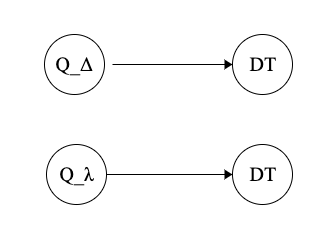
\includegraphics[scale=0.4]{images/DTinstances.png}
\end{center}
To process an incoming stream element, we run our shifting technique on each DT-instance. One with a factor of $\lambda$, the other with a factor of $\Delta$. By our above theorem, we have correctness. \\
\\
To analyse the runtime, we note that $Q_\Delta \cup Q_\lambda = Q$ and $|Q| = m$, so the runtime of either instance is at most $O(n\log m + m\log^2 m \log\tau_{max})$ Hence the total run-time is at most $2\times O(n\log m + m\log^2 m \log\tau_{max}) = \Tilde{O}(n+m)$. This feels a little handwavey but let's move on to something more interesting. \\
\\
Does this generalise further? As before let $Q$ be a set of equal-step queries, though now $Q$ is comprised of queries with $k$ different shift factors; $\Delta_1, \dots, \Delta_k$. As before, we can partition $Q$ into queries of equal shift factor, which we write as $Q_{\Delta_1}, \dots, Q_{\Delta_k}$. As $Q_{\Delta_i}$ are disjoint we have 
$\sum_{i=1}^{k} |Q_{\Delta_i}| = |Q| = m$. As above, we build DT instances on each of the partitions of $Q$. To process an incoming data element, we pass the element through the endpoint tree of $Q_{\Delta_1},\dots, Q_{\Delta_k}$. The total runtime of our algorithm on a stream of $n$ elements is therefore

\begin{align*}
\sum_{i=1}^{k}\text{run-time}(Q_{\Delta_i}) &= \sum_{i=1}^{k} n\log |Q_{\Delta_i}| + |Q_{\Delta_i}|\log^2 |Q_{\Delta_i}| \log\tau_{max} \\
&= \sum_{i=1}^{k} n\log |Q_{\Delta_i}| + \sum_{i=1}^{k}  |Q_{\Delta_i}|\log^2 |Q_{\Delta_i}| \log\tau_{max} 
\end{align*}
Recall the first summation corresponds to the element processing cost, and the latter summation corresponds to the communication cost of each distributed tracking instance. Let's examine the first term
\begin{align*}
    \sum_{i=1}^{k} n\log |Q_{\Delta_i}| &= n\sum_{i=1}^{k}\log |Q_{\Delta_i}| \\
    &= n \log \left(\prod_{i=1}^{k}|Q_{\Delta_i}| \right)
\end{align*}
We can bound the product using the arithmatic mean-geometric mean inqueality which states that: 
$\sqrt[n]{\prod_{i=1}^{n} s_i} \leq \frac{1}{n}\sum_{i=1}^{n}s_i$. Applying to the above we have
\begin{align*}
     n \log \left(\prod_{i=1}^{k}|Q_{\Delta_i}| \right) &\leq n \log\left(
     \frac{1}{k}\sum_{i=1}^{k}|Q_{\Delta_i}|\right)^k \\
     &= n\log^k (m/k \\ 
     &= nk\log (m/k)
\end{align*}
The second summation is a little more trickier to tightly analyse, but we make some simple upper bounds. First, the $\log\tau_{max}$ term in the summation technically corresponds to the maximum threshold among each $Q_{\Delta_{i}}$ set, though clearly each of these will be less than or equaly to the global maximum threshold over all $Q_{\Delta_i}$, so we let $\tau_{max}$ denote this global threshold. Secondly, let $|Q_{\Delta}^*| = \max_{1\leq i \leq k} |Q_{|\Delta_i}|\leq m$ it now follows that 
\begin{align*}
    \sum_{i=1}^{k}  |Q_{\Delta_i}|\log^2 |Q_{\Delta_i}| \log\tau_{max} &\leq \sum_{i=1}^{k}  |Q_{\Delta_i}|\log^2 |Q_{\Delta}^*| \log\tau_{max} \\
    &= m\log^2 |Q_{\Delta}^*| \log\tau_{max} \\
    &\leq m\log^2 m \log\tau_{max}
\end{align*}
Which is the same in terms of big-$O$ as before. This makes sense, as splitting up and processing an element over each of the $k$ DT instances may increase the element processing cost, but it would not alter the total messaging cost of the algorithm. This brings the total runtime analysis to: 

$$O(nk\log (m/k) + m\log^2 m \log\tau_{max})$$
which the worst case depricates to $O(nm)$ runtime. It is now clear that so long as $k = O(\log m)$ we can preserve a runtime of $\Tilde{O}(n+m)$


\newpage
\subsubsection*{Reducing Communication Cost}

Another problem I am looking to study is whether we can reduce communication cost, given that a number of intervals overlap with another. There are two approaches I am looking at tackling with this problem: 
\begin{enumerate}
    \item Theoretically improved bounds with tighter analysis. Having now implemented the endpoint tree in \texttt{C++}, I will look to run experiments on the canoncial node sets of queries when the queries highly overlap, and when they don't. \\
    \\
    If we are able to observe that canconial node sets are themselves overlapping when the intervals are overlapping, we can perhaps improve the theoretical bounds on the communication cost. This would mean we must formalise a notion of \textit{overlapping}, or define a \textit{metric space} on our intervals. This metric can then possibly be used to analyse the communication cost


    \item Design a new data structure. This will require some thought on how it could work, but can we hierarchically \textit{stack} the intervals, so we can easily find all intervals that are stabbed by a given value with ease. The performance of the data structure should improve when the number of intervals overlap. 
\end{enumerate}
\\

\subsubsection*{Implementation}
I have began the implementation in \texttt{C++}, and am making good progress; I plan for this to be completed by the time we meet in Semester 1, 2024. In terms of a To-Do list, I need to develop a series of unit tests, and then rigourously test my implementation. \\
\\
In terms of a performance survey, I have located limit-order-book data sets via \href{https://lobsterdata.com/}{LOBSTER}, which contain a number of free quality academic data sets. These data sets contain negative updates, and should make for an interesting series of experiments. 

\end{document}
